\section{Context}

\begin{frame}{The authors}
    \begin{columns}
        \begin{column}{0.5\textwidth}
            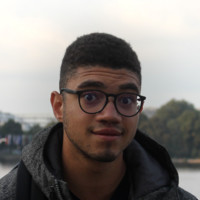
\includegraphics[width = 0.7\textwidth]{images/profile_picture/jeremy.jpeg}
            \begin{itemize}
                \item Jérémy Turi
                \item PhD Student at LAAS-CNRS
                \item Teacher at INSA Toulouse
            \end{itemize}
        \end{column}
        \begin{column}{0.5\textwidth}
            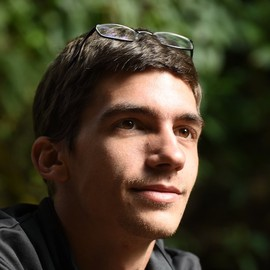
\includegraphics[width = 0.7\textwidth]{images/profile_picture/arthur.jpg}
            \begin{itemize}
                \item Dr. Arthur Bit-Monnot
                \item Researcher at LAAS-CNRS
                \item Associate Professor at INSA Toulouse
            \end{itemize}
        \end{column}
    \end{columns}
\centering
    \begin{itemize}
        \item Part of Robotics \& Interactions Team
    \end{itemize}
\end{frame}

\begin{frame}{The research team}
    Research subjects :
    \begin{itemize}
        \item Human Robot Interaction
        \item Deliberation algorithm and architectures
        \item Planning
        \item Acting
        \item Drones
    \end{itemize}
\end{frame}

\begin{frame}{Scientific interests of the authors}
\begin{itemize}
    \item Study the scalability of existing deliberation algorithms used for single robots for industrial scenarios in multi-agents environments.
    \item Acting algorithms enhanced by decision guidance thanks to planning
    \item My PhD Subject : Planning from operational models for deliberative acting in robotics.
\end{itemize}

\end{frame}

\begin{frame}{The scope of the paper}
    \begin{itemize}
        \item Adapt an existing acting algorithm for multi-agents scenarios dealing with concurrency and shared resources.
        \item The goal of such algorithm :
        \begin{itemize}
            \item monitor and control each agent of the fleet by distributing tasks among them.
            \item Optimize the overall process while taking into account deadlines, contingencies and minimization of resource use.
        \end{itemize}
    \end{itemize}
\end{frame}